%\begin{frame}
%    \frametitle{Übersicht}
%    \begin{columns}
%        \begin{column}{0.50\textwidth}
%            \centering
%            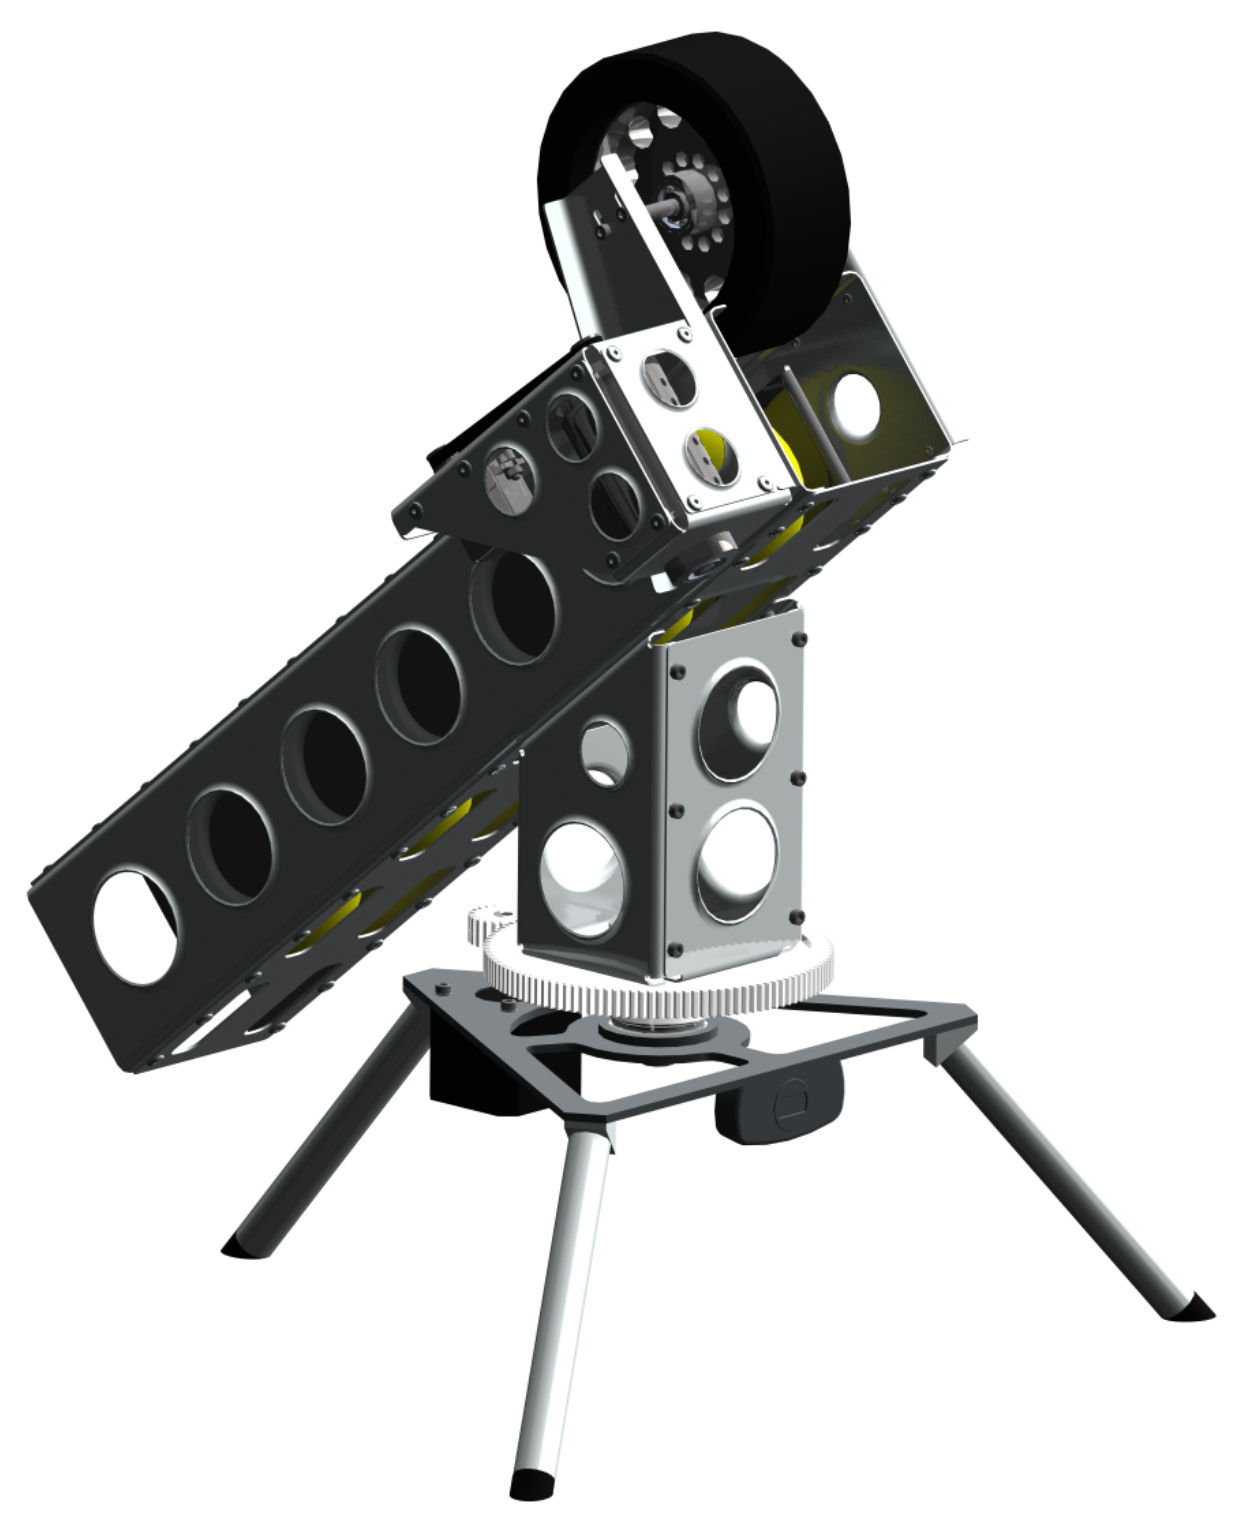
\includegraphics[width=1.00\textwidth]{../doc/fig/Bild_mit_Kamera.png}
%        \end{column}
%        \begin{column}{0.50\textwidth}
%            \begin{block}{Komponenten}
%                \begin{itemize}
%                    \item Kamera
%                    \item Drehvorrichtung
%                    \item Turm
%                    \item Balllager
%                    \item Ballnachschub
%                    \item BLDC Motor
%                \end{itemize}
%            \end{block}
%        \end{column}
%    \end{columns}
%\end{frame}
\begin{frame}
    \frametitle{Übersicht}
    \begin{columns}
        \begin{column}{1.00\textwidth}
            \begin{figure}[h]
                \centering
                \begin{tikzpicture}[scale=1.00]
                    \node[above right] (img) at (0,0) {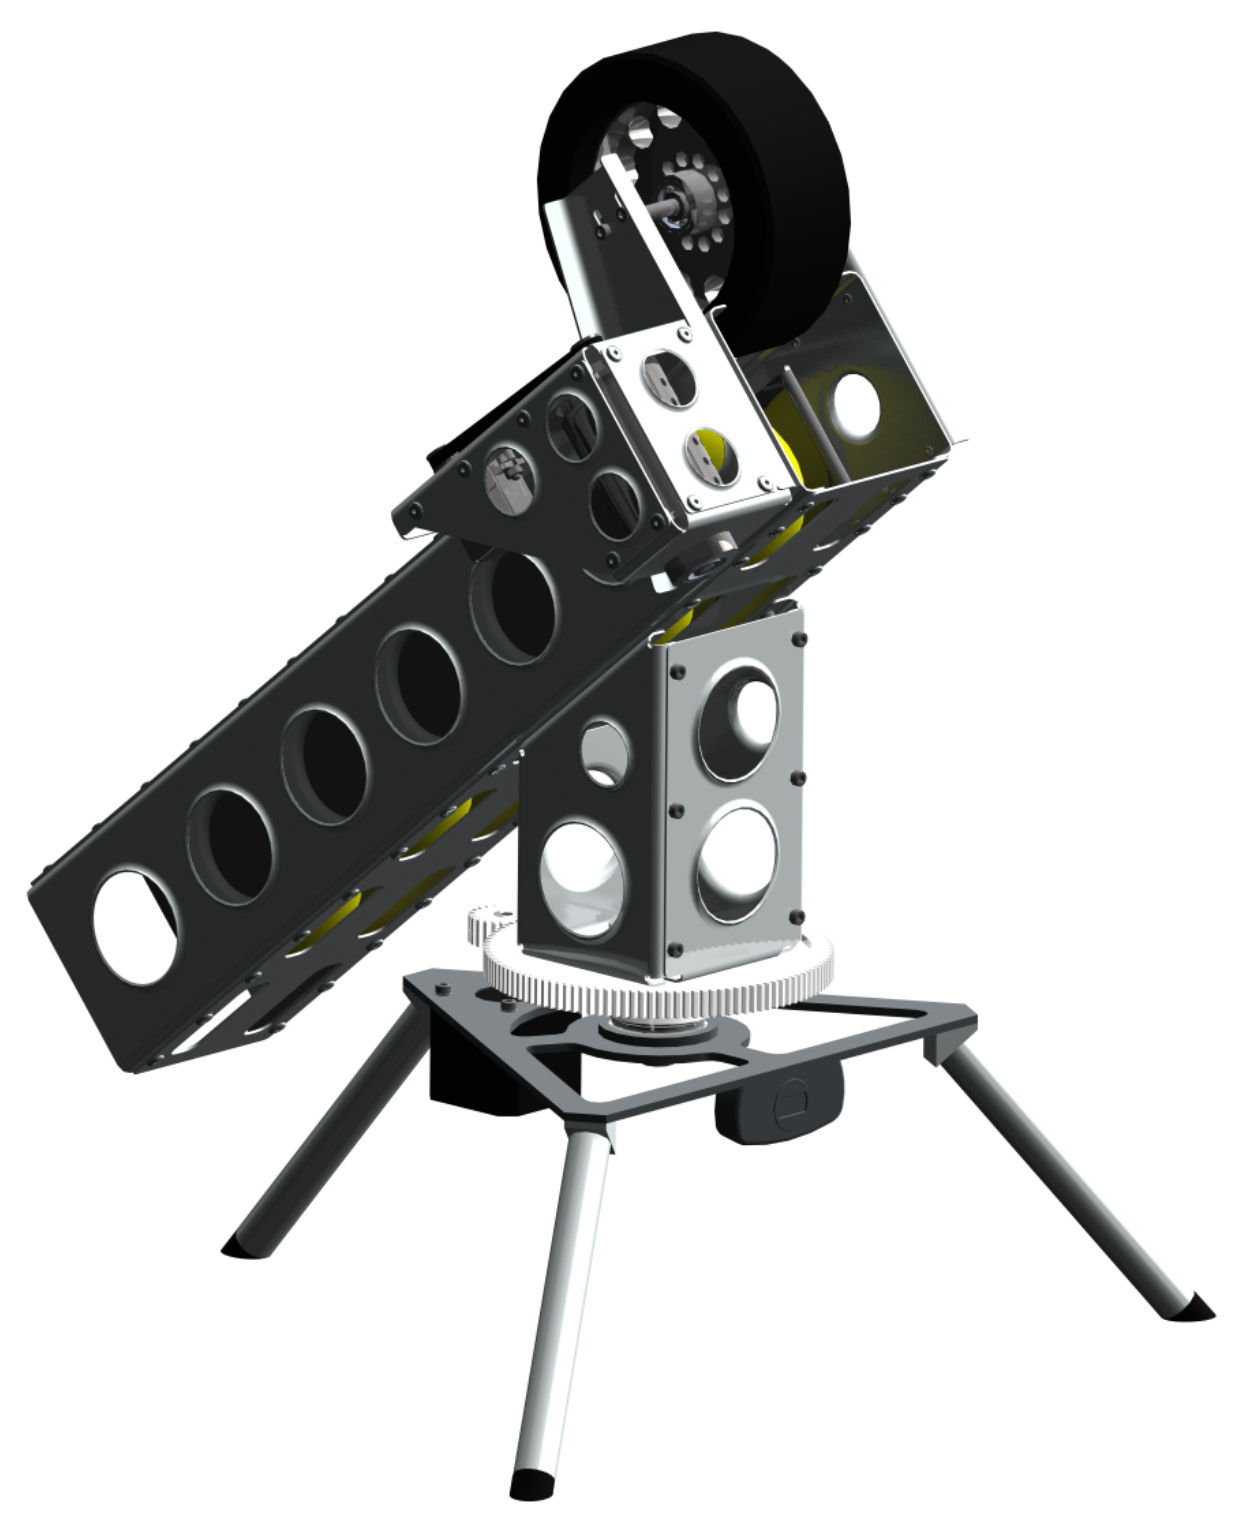
\includegraphics[width=0.50\textwidth]{../doc/fig/Bild_mit_Kamera.png}};
                    \draw[line width=1pt]
                        (0, 4) node[left=0mm] {Balllager}
                        -- (1.5, 3.7);
                    \fill (1.5, 3.7) circle (2pt);
                    \draw[line width=1pt]
                        (1, 5) node[left=0mm] {Ballnachschub}
                        -- (2.5, 4.7);
                    \fill (2.5, 4.7) circle (2pt);
                    \draw[line width=1pt]
                        (6.0, 3.0) node[right=0mm] {Drehvorrichtung}
                        -- (3.0, 2.4);
                    \fill (3.0, 2.4) circle (2pt);
                    \draw[line width=1pt]
                        (5.0, 6.0) node[right=0mm] {BLDC Motor}
                        -- (3.2, 6.0);
                    \fill (3.2, 6.0) circle (2pt);
                    \draw[line width=1pt]
                        (5.5, 4.5) node[right=0mm] {Turm}
                        -- (3.5, 3.5);
                    \fill (3.5, 3.5) circle (2pt);
                    \draw[line width=1pt]
                        (6.5, 1.5) node[right=0mm] {Kamera}
                        -- (3.7, 2.0);
                    \fill (3.7, 2.0) circle (2pt);
                \end{tikzpicture}
            \end{figure}
        \end{column}
    \end{columns}
\end{frame}

